\section[搜索定位接收机]{搜索定位接收机\\Receiver Position by Search}
	我们描述一个搜索过程,解决了最小二乘问题没有形成正常的方程。假设四个或更多伪距美元$P_1,P_2,\vdots,P_m$在同一历元。我们要确定我们的接收机的位置,没有先验知识,它的位置。
		
	首先我们计算ECEF坐标的m卫星星历文件。然后wc的笛卡尔坐标变换每个卫星传输时间(可以从伪距获得)到 $(\varphi_i,\lambda_i)$ = (纬度,经度)。平均坐标是我们第一次猜的接收机的位置。
		
	以这个点为中心,我们引入一个网格覆盖一个半球。可能将$\pi/2$十等分,可能16等分$2\pi$的角度。在每个网格点,我们计算剩余 $R_i=P_i-P_1,i=2,\vdots,m $,观察到的伪距之间的差异和第一个值来消除接收机时钟偏移量。接下来我们区分这些差异:
	\begin{align*}
		r_1& = R_2-R^0_2 = (P_2-P_1) - (P^0_2-P^0_1) \\
		r_2& = R_3-R^0_3 = (P_3-P_1) - (P^0_3-P^0_1) \\
		\vdots& \\
		r_{m-1}& = R_m-R^0_m = (P_m-P_1) - (P^0_m-P^0_1) 
	\end{align*}
	\begin{figure}
			\centering
			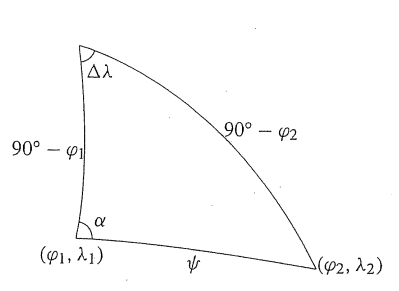
\includegraphics[width=0.7\linewidth]{TeX_files/Part03/chapter09/image/9-15}
			\caption{球面三角形计算接收机的纬度和经度 $(\varphi,\lambda)$}
			\label{fig:9-15}
	\end{figure}

	这给第一个近似和$S=\Sigma r^2_i$之间的所有S的可能值,现我们寻求最小的一个,现与该值是新的接收机的位置的估计值。网格是为更精细的下一次迭代。现一个新的决定和选择如下,细化网格的中心和一个后续的搜索。重复这个过程,直到没有进一步改善位置。

	最后,我们展示如何计算球面三角学的新位置,如图\ref{fig:9-15}。最初点的坐标 $(\varphi_1,\lambda_1)$。我们想要移动$\psi$度沿方位角$(\varphi_2,\lambda_2)$的方向。计算$\varphi_2$和$\lambda_2$是一个经典大地测量问题,以下基本方程产生解决方案在球面上:
	\begin{equation}\label{eq:9.32}
		\sin\varphi_2 = \sin\varphi_1\cos\psi+\cos\varphi_1\sin\psi\cos\alpha\quad and \quad \sin\Delta\lambda=\dfrac{\sin\aleph\sin\psi}{\cos\varphi_2}
	\end{equation}

	这些方程给出新的点的纬度 $\varphi_2$和增量$\Delta\lambda$的经度。的m文件recpos显示了快速的实现代码。最终找到一个接收器位置与轨道的精度一致,折射模型和伪距。
		
	这是另一个最小二乘的一个例子。这里,由于$P_1$减去其他伪距,这显然是相关的差异。任何错误在$P_1$出现在每一个差异中。在搜索中我们忽略这些相关性,因为这个过程只是为了给第一次估计的接收机的位置。
		
	使用适当的协方差矩阵最小二乘过程应该遵循我们的搜索技术。由此产生的猜测是几乎总是(线性)收敛区域内。获得的导航数据rinexe $('ohiostat.96n','rinex_n.dat')$。你可以放大图片按下鼠标按钮。许多你可以读出缩放后的x和y标签的位置。

	将$get_eph$m文件打开,读取和构造一个星历表文件。这样的文件通常包含几个特定卫星数据集。常见的做法是选择立即时代之前的星历表使用。文件$find_eph$便是这个用途。然而保持这种做法,最终导致星历数据的变化。这很可能会引入跳轨道计算。更先进的程序平滑轨道,如果他们需要更长时间的使用。一个更好的解决方案是改用精密星历表。
